\documentclass[12pt, legalpaper]{exam}
\usepackage[utf8]{inputenc}
\usepackage[english]{babel}
\usepackage[margin=.8in]{geometry}
\usepackage{amsmath,amssymb}
\usepackage{multicol}
\usepackage{graphicx}
\usepackage{tikz}
\usepackage{lastpage}
\usepackage{tabularx}
\usepackage{hyperref}
\usepackage{tcolorbox}
\newcommand{\course}{Introduction to Optimization}
\newcommand{\term}{Fall 2023}
\newcommand{\examnum}{Report of Programming Task 3}


\usepackage{listings}

\begin{document}
\noindent \examnum \, of the  course ''\course'' - \term


\noindent
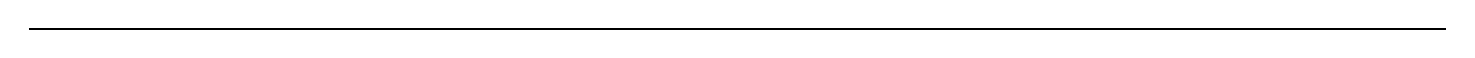
\begin{tikzpicture}
\draw[thick] (0,0) -- (18,0);
\end{tikzpicture}




\vspace{12pt}
\begin{center}
    \textbf{Report 3}
\end{center}
% \noindent \textbf{Requirements}

\vspace{12pt}

\noindent  \textbf{Team information.}

\begin{itemize}
    \item Team leader: Ilia Mitrokhin
    \item Team member 1: Max Martyshov
    \item Team member 2: Mintimer Karimov
    \item Team member 3: Kirill Arkhipov
    \item Team member 4: Timur Zheksimbaev
    \item Team member 5: Aleksandr Ryabov
\end{itemize}
\vspace{12pt}
\noindent     \textbf{Link to the product.}
\begin{itemize}
    \item The product is available: 
    
    \url{https://github.com/paket2004/ProgTask3}
\end{itemize}

\vspace{12pt}

\noindent  \textbf{Programming language.}
\begin{itemize}
    \item Programming language: Python
\end{itemize}

\vspace{12pt}

\noindent  \textbf{Transportation Problem.}

Given balanced Transportation Problem that has 3 sources and 4 destinations.

- A vector of coefficients of supply
$$ (160 \: 140 \: 170) $$

- A matrix of coefficients of costs
$$ 
    \begin{pmatrix}
        7 & 8 & 1 & 2\\
        4 & 5 & 9 & 8\\
        9 & 2 & 3 & 6
    \end{pmatrix}
$$

- A vector of coefficients of demand 
$$ (120 \: 50 \: 190 \: 110) $$

\noindent     \textbf{Input}

\vspace{12pt}
The input contains:
\begin{itemize}
    \item A vector of coefficients of supply - $S$
    \item A matrix of coefficients of costs - $C$
    \item A vector of coefficients of demand - $D$
\end{itemize}

\vspace{12pt}
\textbf{Example of input:}
\begin{verbatim}
    s = [160, 140, 170]

    c = [
        [7, 8, 1, 2],
        [4, 5, 9, 8],
        [9, 2, 3, 6],
    ]

    d = [120, 50, 190, 110]
\end{verbatim}

\vspace{12pt}
\noindent     \textbf{Output/Results}

The output contains table definition of of given Transportation Problem
and its solutionderived with following methods:

\begin{itemize}
    \item North-West Corner Method
    \item Vogel`s Approximation Method
    \item Russell`s Approximation Method
\end{itemize}

\vspace{12pt}
\textbf{Example of output:}

\begin{verbatim}
    ---------------------------
        | 0  | 1  | 2  | 3  | Supply
    ---------------------------
    0      |    |    |    |    | 160
    1      |    |    |    |    | 140
    2      |    |    |    |    | 170
    ---------------------------
    Demand |120 | 50 |190 |110 |

    North-West Corner Method
    ---------------------------
        | 0  | 1  | 2  | 3  | Supply
    ---------------------------
    0      |120 |    |    |    | 40
    1      | 20 | 50 |    |    | 120
    2      |    | 50 |190 |    | 140
    ---------------------------
    Demand |   |    |    |110 |

    Total: 2270

    Vogel`s Approximation Method
    ---------------------------
        | 0  | 1  | 2  | 3  | Supply
    ---------------------------
    0      |120 |    |    |    | 40
    1      |    | 50 |    |    | 100
    2      |    |    |190 |    | 170
    ---------------------------
    Demand |   |    |    |110 |

    Total: 2070

    Russell`s Approximation Method
    ---------------------------
        | 0  | 1  | 2  | 3  | Supply
    ---------------------------
    0      |120 |    |    |    | 40
    1      |    | 50 |    |    | 100
    2      |    |    |190 |    | 170
    ---------------------------
    Demand |   |    |    |110 |

    Total: 2070
\end{verbatim}

\noindent
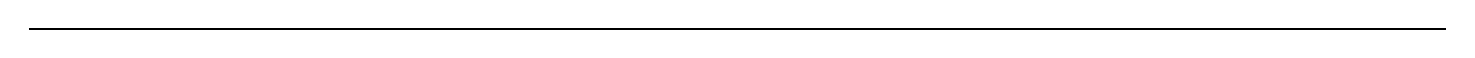
\begin{tikzpicture}
\draw[thick] (0,0) -- (18,0);
\end{tikzpicture}




\clearpage
\noindent     \textbf{Code of the program:}


\begin{lstlisting}{Python}
    def north_west(s: list[int], c: list[list[int]], d: list[int])
                     -> list[list[int]]:
    # Copy input data to avoid modifying the original lists
    s = s.copy()
    c = [i.copy() for i in c]
    d = d.copy()

    # Initialize the result matrix with zeros
    res = [[0] * len(i) for i in c]

    # Perform the North-West corner method
    i = j = 0
    while i < len(s) and j < len(d):
        
    # Step 1: Select the upper-left cell of the transportation
        # matrix and assign the  #minimum value of supply or
        # demand, i.e., min(supply, demand).

        mn = min(s[i], d[j])
        res[i][j] = mn
        
        # Subtract the above minimum value from supply 
        # or demand of the corresponding row and column.
        
        s[i] -= mn
        d[j] -= mn
        
        # We may get 3 possibilities:
        
        # If the supply is equal to 0, 
        # strike that row and move down to the next cell.
        
        # If the demand equals 0,
        # strike that column and move right to the next cell.

        # If supply and demand are 0, 
        # then strike both row and column 
        # and move diagonally to the next cell.
        i += (s[i] == 0)
        j += (d[j] == 0)
        
        # Repeat until all the values
        # will be equal to zero (supply and demand).

    return res


def vogel(s: list[int], c: list[list[int]], d: list[int]) 
            -> list[list[int]]:

    # Copy input data to avoid modifying the original lists
    s = s.copy()
    c = [i.copy() for i in c]
    d = d.copy()

    # Initialize the result matrix with zeros
    res = [[0] * len(i) for i in c]

    # Calculate the total supply
    total = sum(s)

    # Perform Vogel's approximation method
    while total:
        # Initialize a list to store priority information
        priorities = []
        
        # Calculate the penalty for each row
        for i in range(len(s)):
            if not s[i]: continue
            v = sorted((c[i][j], (i, j)) for j in range(len(d)))
            row = (v[1][0] - v[0][0], -v[0][0], v[0][1])
            priorities.append(row)
        
            # Calculate the penalty for each column
        for j in range(len(d)):
            if not d[j]: continue
            v = sorted((c[i][j], (i, j)) for i in range(len(s)))
            row = (v[1][0] - v[0][0], -v[0][0], v[0][1])
            priorities.append(row)

        # Find the cell with the maximum penalty
        i, j = max(priorities)[2]
        
        # Determine the minimum quantity to transport
        mn = min(s[i], d[j])

        # Update the result matrix, supplies, and demands
        total -= mn
        res[i][j] = mn
        s[i] -= mn
        d[j] -= mn

        # Mark rows or columns with exhausted supplies or demands
        if s[i] == 0:
            for J in range(len(d)): c[i][J] = float('inf')
        if d[j] == 0:
            for I in range(len(s)): c[I][j] = float('inf')

    return res


def russel(s: list[int], c: list[list[int]], d: list[int]) 
            -> list[list[int]]:

    # Copy input data to avoid modifying the original lists
    s = s.copy()
    c = [i.copy() for i in c]
    d = d.copy()

    # Initialize the result matrix with zeros
    res = [[0] * len(i) for i in c]

    # Calculate the rows and columns with maximum values
    rows = [max(c[i][j] for j in range(len(d))) 
            for i in range(len(s))]
    columns = [max(c[i][j] for i in range(len(s)))
                 for j in range(len(d))]

    # Create a list of priorities based 
    # on the difference between costs and maximum values
    priorities = sorted(
        (c[i][j] - rows[i] - columns[j], c[i][j], (i, j)) 
        for j in range(len(d)) for i in range(len(s))
        )

    # Perform Russell's approximation method
    for _, _, (i, j) in priorities:
        
        # Find the minimum of available supply 
        # at i-th source and demand at j-th destination
        mn = min(s[i], d[j])
        
        # Allocate the minimum amount in the result matrix
        # at the i-th source and j-th destination
        res[i][j] = mn
        
        # Update the remaining supply and demand after allocation
        s[i] -= mn
        d[j] -= mn

    return res


def check():
    # Check if the problem is balanced and the method is applicable
    if sum(s) != sum(d):
        print("The problem is not balanced!")
        exit()
    if min(min(i) for i in c) <= 0:
        print("The method is not applicable!")
        exit()
    if len(c) != len(s):
        print("The method is not applicable!")
        exit()
    if any(len(i) != len(d) for i in c):
        print("The method is not applicable!")
        exit()


def print_table(res: list[list[int]] = None, name: str = "Initial") 
                    -> None:

    # Print the transportation table
    res = res or [[0] * len(i) for i in c]
    res = [[(f'({b}) ' if b else '') + str(j)
     for j, b in zip(i, a)] for i, a in zip(c, res)]
    
    l = max(6, max(len(max(i, key=len)) for i in res)) + 3
    ln = l * (len(d) + 2) + 2
    
    print(("{:^" + f'{ln}' + "}").format(name))
    print('-' * ln)
    
    frmt = "{:>" + f'{l}' + "}"
    
    print(frmt.format(''), end='|')
    print((frmt * len(d)).format(*range(len(d))), end='|')
    print(frmt.format('Supply'))
    print('-' * ln)
    
    for i in range(len(s)):
        print(frmt.format(str(i)), end='|')
        print((frmt * len(d)).format(*res[i]), end='|')
        print(frmt.format(s[i]))
    
    print('-' * ln)
    print(frmt.format('Demand'), end='|')
    print((frmt * len(d)).format(*d), end='|\n')


def print_total(res: list[list[int]]) -> None:
    # Print the total cost of transportation
    print(f'Total: {sum(sum(j * b for j, b in zip(i, a)) 
            for i, a in zip(c, res))}')


# Input data
s = [160, 140, 170]
c = [
    [7, 8, 1, 2],
    [4, 5, 9, 8],
    [9, 2, 3, 6],
]
d = [120, 50, 190, 110]

# Check the input data
check()

# Print the initial transportation table
print_table()

# Apply transportation methods and print the results
for method, name in zip((north_west, vogel, russel),
                        ('North-West corner method',
                         'Vogel`s approximation method',
                          'Russell`s approximation method')):
    print()
    res = method(s, c, d)
    print_table(res, name)
    print_total(res)
    
\end{lstlisting}

\end{document}
